\documentclass{6033dp1/6033dp1}
\usepackage{graphicx}

\title{6.033 Design Project 2}
\author{Andrew Cooper\\ William Stueck\\ Patrick Vatterott}
\recitation{Recitation 06}

\begin{document}
\maketitle

\section{Introduction}
CVS, named for its creators Cooper, Vatterott, and Stueck, is a peer to peer text editor.  The system is designed to operate in a distributed network where all users are not necessarily always connected, and where no central server is used to host the developing document.  CVS is designed, in particular, for situations where users connect their laptops to each other, but may not necessarily all be connected at the same time, and may never connect over the internet.  CVS employs a set of clever safety mechanisms and data storage techniques to ensure that all users can seamlessly operate on a document without doing unnecessary work.

\section{Data Structure}
The document is stored on disk in the form of a tree.  The root of the tree represents the document as a whole, and the document�s inode holds a pointer to this location on disk.  This location on disk, in turn, knows how many paragraphs the document contains, and contains pointers to each of the document�s paragraphs.  At the next level in the tree, each paragraph contains pointers to each sentence.  Finally, each sentence in the tree actually contains the data of individual sentences.  The concept of the tree is just a way of representing the data of a document.  By choosing to represent data in this manner, tasks such as merging and commiting code can be done in a very efficient manner.  Consider the following document. \\[18px]
\textit{The dog runs. The dog is fast.}\\[12px]
\textit{The cat naps.}\\[18px]
The previous document can be seen in Figure 1, in the form of the data structure that represents the document.

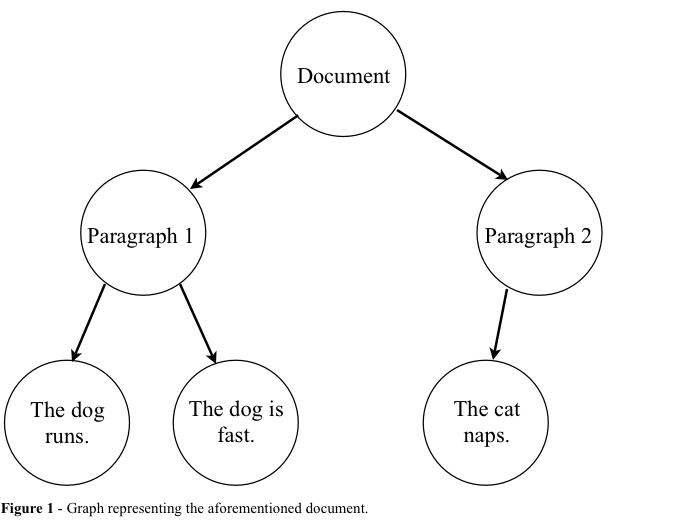
\includegraphics[scale=0.70]{graph1.png}

\section{Version Vector}
A document's version information is represented in a modified version vector
maintained by each user. Each paragraph in the document is assigned a unique
paragraph id. The vector contains (paragraph id, version number)
pairs, ordered so that each paragraph occurs in the vector in the order it occurs
in the document. Every time a user merges his changes with another user, both save
the vector they have agreed upon.

$$
 [ (pid, version), (pid, version), (pid, version) ]
$$

This allows the system to track changes to individual paragraphs as well as changes
to the order of paragraphs. If for example, in a document with three paragraphs, 
A moves paragraph 1 to the end, and B changes a word in paragraph 1, their vectors
will change from:

$$ 
 A, B: [ (1, 0), (2, 0), (3, 0) ]
$$

to:

$$
 A: [ (2, 0), (3, 0), (1, 0) ] $$ $$ 
 B: [ (1, 1), (2, 0), (3, 0) ]
$$

upon merging, both users will see that the vectors are different than the last
agreed upon vector, and the merging process will occur. Because of how the vector
is structured, only the text from one paragraph needs to be transmitted between 
hosts, the order information can be transmitted using a more concise protocol.



\section{Merging}
Merging will occur when two or more users have changed the same document. The design will handle both automatic and manual merging, where manual merging will require the user to correct the merging conflicts themselves.
%\vspace{12 pt} \\

As seen above, each text document will be stored as a tree where parents correspond to paragraphs and children correspond to sentences. The version vectors stored for each document will keep track of the modifications to individual paragraphs between peers. Automatic merging will take place when peers have made changes to different paragraphs because these changes will not interfere with one another. When users modify the same paragraph in a document, the system must traverse the tree and analyze individual sentences. Using an insert, delete, and modify algorithm, the system will be able to determine the modifications among the sentences within the paragraph and any conflicts that emerged due to the modifications. Depending on the change, the system can either automatically merge the documents or alert the users of a conflict that must be merged manually.
%\vspace{12 pt} \\

\section{Commit Points}
The P2P text editor must be able to support commit points. A commit point is defined as a point in time when a user can manually commit the current version of a text file, and once every user agrees on the commit, that current state of the text file is preserved on all systems.  This functionality allows users to save previous versions of a file and also allows them to have a file backup in the event of a system crash.

%\vspace{12 pt} \\
Whether offline or online, when a user makes a commit, a new file is created on his/her system. The file is named in the following manner: \emph{oldFileName\_commitName.txt}. \emph{oldFileName} refers to the name of the original file, and \emph{commitName} refers to the name of the commit submitted by the user. The next time that user comes online, the system will talk to all peers to see if changes have been made to the committed file. If no changes have been made, the commit is a success, and \emph{oldFileName\_commitName.txt} is saved on every user's machine. If changes have been made, the commit fails. The system then follows the merging process described above to update any changes to \emph{oldFileName\_commitName.txt}, and that new state is saved on every user's machine. Assuming $n$ commits between peers, the a user's system should have $n+1$ files associated with the text document.
%\vspace{12 pt} \\


\section{Conclusion}

ipsum lorum

\end{document}
